\subsection{Obtención de los Requisitos del Sistema} 

\subsubsection{Requisitos de interfaces externas}

\paragraph*{Interfaces de usuario}
\newlist{myEnumIU}{enumerate}{4}
\setlist[myEnumIU,1]{label=\textbf{RIE-IU-\arabic*.}}
\setlist[myEnumIU,2]{label*=\textbf{\arabic*.}}
\setlist[myEnumIU,3]{label*=\textbf{\arabic*.}}
\setlist[myEnumIU,4]{label*=\textbf{\arabic*.}}
\begin{myEnumIU}
	\item El sistema será accesible desde cualquier dispositivo que cuente con conexión a internet y un navegador web.
	\item El sistema estará disponible en diferentes idiomas.
	\begin{myEnumIU}
		\item Español
		\item Inglés
	\end{myEnumIU}
	\item El sistema deberá ser accesible para todos los usuarios a través de los navegadores más comunes.
	\begin{myEnumIU}
		\item Google Chrome
		\item Mozilla Firefox
		\item Microsoft Edge
	\end{myEnumIU}
	\item El usuario podrá utilizar todas las funcionalidades desarrolladas de la aplicación sin inconvenientes.
	\item El usuario no necesitará de conocimientos tecnológicos avanzados.
\end{myEnumIU}

\paragraph*{Interfaces hardware}
\newlist{myEnumIH}{enumerate}{4}
\setlist[myEnumIH,1]{label=\textbf{RIE-IH-\arabic*.}}
\setlist[myEnumIH,2]{label*=\textbf{\arabic*.}}
\setlist[myEnumIH,3]{label*=\textbf{\arabic*.}}
\setlist[myEnumIH,4]{label*=\textbf{\arabic*.}}
\begin{myEnumIH}
	\item El sistema dispondrá de una base de datos para almacenar la información necesaria.
\end{myEnumIH}

%\paragraph*{Interfaces software}

\paragraph*{Interfaces de comunicaciones}
\newlist{myEnumIC}{enumerate}{4}
\setlist[myEnumIC,1]{label=\textbf{RIE-IC-\arabic*.}}
\setlist[myEnumIC,2]{label*=\textbf{\arabic*.}}
\setlist[myEnumIC,3]{label*=\textbf{\arabic*.}}
\setlist[myEnumIC,4]{label*=\textbf{\arabic*.}}
\begin{myEnumIC}
	\item El sistema contendrá enlaces a diferentes sitios web.
	\item El sistema mostrará por defecto enlaces a los siguientes sitios web.
	\begin{myEnumIC}
		\item Twitter oficial de la Escuela de Ingeniería Informática
		\item Página web de la Escuela de Ingeniería Informática
		\item Página web de la Universidad de Oviedo
	\end{myEnumIC}
\end{myEnumIC}


\subsubsection{Requisitos funcionales}
\newlist{myEnumRF}{enumerate}{2}
\setlist[myEnumRF,1]{label=\textbf{RF-\arabic*.}}
\setlist[myEnumRF,2]{label*=\textbf{\arabic*.}}
\begin{myEnumRF}
	\item El sistema estará constituido por dos aplicaciones web diferentes.
	\begin{myEnumRF}
		\item El museo.
		\item La administración del museo.
	\end{myEnumRF}
\end{myEnumRF}

\paragraph*{Museo}
\newlist{myEnumRFM}{enumerate}{9}
\setlist[myEnumRFM,1]{label=\textbf{RF-MU-\arabic*.}}
\setlist[myEnumRFM,2]{label*=\textbf{\arabic*.}}
\setlist[myEnumRFM,3]{label*=\textbf{\arabic*.}}
\setlist[myEnumRFM,4]{label*=\textbf{\arabic*.}}
\setlist[myEnumRFM,5]{label*=\textbf{\arabic*.}}
\setlist[myEnumRFM,6]{label*=\textbf{\arabic*.}}
\setlist[myEnumRFM,7]{label*=\textbf{\arabic*.}}
\setlist[myEnumRFM,8]{label*=\textbf{\arabic*.}}
\setlist[myEnumRFM,9]{label*=\textbf{\arabic*.}}
\begin{myEnumRFM}
	\item El sistema mostrará los periodos existentes.
	\begin{myEnumRFM}
		\item Los periodos estarán ordenados por año de inicio.
		\item Se presentarán en una línea temporal incluyendo los siguientes datos.
		\begin{myEnumRFM}
			\item Nombre.
			\item Año de inicio.
			\item Año de fin.
			\item Nombres de los componentes pertenecientes al periodo.
		\end{myEnumRFM}
	\end{myEnumRFM}
	\item El sistema permitirá realizar búsquedas.
	\begin{myEnumRFM}
		\item Se podrá buscar por los siguientes campos.
		\begin{myEnumRFM}
			\item Por nombre.
			\item Por un intervalo de años.
		\end{myEnumRFM}
		\item Al realizar la búsqueda se mostrará la línea temporal filtrada con los resultados.
	\end{myEnumRFM}
	\item\label{it:detalles_periodo} El sistema mostrará los detalles de un periodo.
	\begin{myEnumRFM}
		\item Nombre.
		\item Características.
		\item Listado de datos curiosos (Sabías qué...).
		\item Eventos ocurridos durante el periodo.
		\item Sistemas famosos que contienen componentes de este periodo.
		\item Listado de los componentes pertenecientes al periodo.
	\end{myEnumRFM}
	\item\label{it:detalles_comp} El sistema mostrará los detalles de un componente.
	\begin{myEnumRFM}
		\item Nombre.
		\item Descripción.
		\item Imágenes.
		\item Año de inicio.
		\item Año de fin.
		\item Precio.
		\item Tipo de dispositivos en los que se encuentra.
		\begin{myEnumRFM}
			\item Portátiles.
			\item De escritorio.
		\end{myEnumRFM}
		\item Detalles específicos del tipo de componente.
		\begin{myEnumRFM}
			\item Detalles de CPU.
			\begin{myEnumRFM}
				\item Memoria ROM (obligatorio).
				\item Memoria RAM (obligatorio).
				\item Velocidad de reloj (obligatorio).
				\item Potencia (obligatorio).
				\item Tamaño de palabra (obligatorio).
				\item Nanómetros de los transistores (obligatorio).
				\item Passmark (obligatorio).
				\item Número de transistores (obligatorio).
			\end{myEnumRFM}
		\end{myEnumRFM}
	\end{myEnumRFM}
\end{myEnumRFM}

\paragraph*{Administración del museo}
\newlist{myEnumRFA}{enumerate}{9}
\setlist[myEnumRFA,1]{label=\textbf{RF-ADM-\arabic*.}}
\setlist[myEnumRFA,2]{label*=\textbf{\arabic*.}}
\setlist[myEnumRFA,3]{label*=\textbf{\arabic*.}}
\setlist[myEnumRFA,4]{label*=\textbf{\arabic*.}}
\setlist[myEnumRFA,5]{label*=\textbf{\arabic*.}}
\setlist[myEnumRFA,6]{label*=\textbf{\arabic*.}}
\setlist[myEnumRFA,7]{label*=\textbf{\arabic*.}}
\setlist[myEnumRFA,8]{label*=\textbf{\arabic*.}}
\setlist[myEnumRFA,9]{label*=\textbf{\arabic*.}}
\begin{myEnumRFA}
	\item El sistema permitirá al usuario iniciar sesión mediante un formulario.
	\begin{myEnumRFA}
		\item El formulario se solicitan los siguientes campos.
		\begin{myEnumRFA}
			\item Correo electrónico (obligatorio).
			\item Contraseña (obligatorio).
		\end{myEnumRFA}
		\item Si los campos no son correctos, se mostrará de nuevo el inicio de sesión.
		\item Si los campos son válidos, se accederá al sistema como administrador.
	\end{myEnumRFA}
%	\item El sistema permitirá al usuario modificar la contraseña.
	\item El sistema mostrará un listado de los periodos existentes.
	\item El sistema mostrará los detalles de un periodo.
	\begin{myEnumRFA}
		\item Especificados en \ref{it:detalles_periodo}
	\end{myEnumRFA}
	\item El sistema mostrará los detalles de un componente.
	\begin{myEnumRFA}
		\item Especificados en \ref{it:detalles_comp}
	\end{myEnumRFA}
	\item El sistema permitirá añadir un periodo.
	\begin{myEnumRFA}
		\item\label{it:campos_periodo} Se introducirán los datos mediante un formulario con los siguientes campos.
		\begin{myEnumRFA}
			\item Nombre (obligatorio).
			\item Características (obligatorio).
			\item Listado de datos curiosos (Sabías qué...) (obligatorio).
			\item Eventos ocurridos durante el periodo (obligatorio).
		\end{myEnumRFA}
	\end{myEnumRFA}
	\item El sistema permitirá añadir un componente a un periodo existente.
	\begin{myEnumRFA}
		\item\label{it:campos_comp} Se introducirán los datos mediante un formulario con los siguientes campos.
		\begin{myEnumRFA}
			\item Nombre (obligatorio).
			\item Tipo de componente (obligatorio).
			\begin{myEnumRFA}
				\item CPU.
			\end{myEnumRFA}
			\item Descripción (obligatorio).
			\item Familia de componente (obligatorio).
			\item Imágenes.
			\item Año de inicio (obligatorio).
			\item Año de fin (obligatorio).
			\item Precio (obligatorio).
			\item Tipo de dispositivos en los que se encuentra.
			\begin{myEnumRFA}
				\item Portátiles.
				\item De escritorio.
			\end{myEnumRFA}
			\item Sistema famoso que lo contiene.
			\begin{myEnumRFA}
				\item Nombre del sistema.
				\item Imagen del sistema.
			\end{myEnumRFA}
			\item Detalles específicos del tipo de componente.
			\begin{myEnumRFA}
				\item Detalles de CPU.
				\begin{myEnumRFA}
					\item Memoria ROM (obligatorio).
					\item Memoria RAM (obligatorio).
					\item Velocidad de reloj (obligatorio).
					\item Potencia (obligatorio).
					\item Tamaño de palabra (obligatorio).
					\item Nanómetros de los transistores (obligatorio).
					\item Passmark (obligatorio).
					\item Número de transistores (obligatorio).
				\end{myEnumRFA}
			\end{myEnumRFA}
		\end{myEnumRFA}
	\end{myEnumRFA}
	\item El sistema permitirá editar periodos.
	\begin{myEnumRFA}
		\item Se introducirán los datos mediante un formulario.
		\begin{myEnumRFA}
			\item Campos especificados en \ref{it:campos_periodo}
		\end{myEnumRFA}
	\end{myEnumRFA}
	\item El sistema permitirá editar componentes.
	\begin{myEnumRFA}
		\item Se introducirán los datos mediante un formulario.
		\begin{myEnumRFA}
			\item Campos especificados en \ref{it:campos_comp}
		\end{myEnumRFA}
	\end{myEnumRFA}
	\item El sistema permitirá eliminar un periodo.
	\begin{myEnumRFA}
		\item Se pedirá confirmación antes de eliminarlo.
		\item Se eliminarán los componentes pertenecientes a dicho periodo.
	\end{myEnumRFA}
	\item El sistema permitirá eliminar un componente.
	\begin{myEnumRFA}
		\item Se pedirá confirmación antes de eliminarlo.
	\end{myEnumRFA}
\end{myEnumRFA}


%\subsubsection{Requisitos de rendimiento}
%\subsubsection{Requisitos lógicos de BD}
%\subsubsection{Requisitos de desarrollo}
%\subsubsection{Restricciones de diseño}
\subsubsection{Atributos del sistema}

\paragraph*{Seguridad}
\newlist{myEnumSEG}{enumerate}{2}
\setlist[myEnumSEG,1]{label=\textbf{RNF-SEG-\arabic*.}}
\setlist[myEnumSEG,2]{label*=\textbf{\arabic*.}}
\begin{myEnumSEG}
	\item La parte de administración del sistema se asegurará de que el usuario se identifica para acceder a ella.
	\begin{myEnumSEG}
		\item El usuario se identificará mediante un email y una contraseña.
	\end{myEnumSEG}
	\item El sistema cifrará la contraseña para almacenarla en la base de datos.
\end{myEnumSEG}


\subsection{Identificación de Actores del Sistema} 
\subsubsection{Usuario estándar}
Actor que interactúa con el sistema. Tiene acceso de lectura a la página web del museo. Solo debe tener un conocimiento básico para navegar por internet.
\subsubsection{Usuario administrador}
Actor que interactúa con el sistema. Debe iniciar sesión en la parte de administración del sistema, es el único actor con acceso a esta. Es responsable de gestionar el sistema y su mantenimiento. Debe tener amplios conocimientos sobre el sistema.

\subsection{Especificación de Casos de Uso}

\begin{figure}[H]
\centering
\centerline{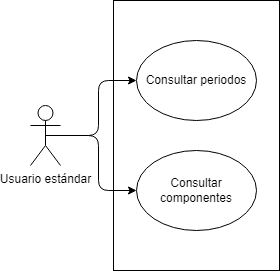
\includegraphics[scale=0.7]{casos-uso-museo}}
\caption{Diagrama de casos de uso del museo}
\end{figure}

\begin{table}[htbp]
  \centering
  \caption{Especificación Caso de Uso 1}
    \begin{tabular}{p{20.855em}r}
\cmidrule{1-1}    \rowcolor[rgb]{ .949,  .949,  .949} \multicolumn{1}{p{20.855em}}{\textbf{Nombre del caso de uso}} & \multicolumn{1}{r}{\cellcolor[rgb]{ 1,  1,  1}} \\
\cmidrule{1-1}    \multicolumn{1}{p{20.855em}}{Consultar periodos} & \multicolumn{1}{r}{} \\
    \midrule
    \rowcolor[rgb]{ .949,  .949,  .949} \multicolumn{2}{p{31.64em}}{\textbf{Descripción}} \\
    \midrule
    \multicolumn{2}{p{31.64em}}{Un usuario estándar puede visualizar los periodos existentes en el museo.} \\
    \bottomrule
    \end{tabular}%
  \label{espec_caso_uso_1}%
  \vspace{-4mm}
\end{table}%

\begin{table}[htbp]
  \centering
  \caption{Especificación Caso de Uso 2}
    \begin{tabular}{p{20.855em}r}
\cmidrule{1-1}    \rowcolor[rgb]{ .949,  .949,  .949} \multicolumn{1}{p{20.855em}}{\textbf{Nombre del caso de uso}} & \multicolumn{1}{r}{\cellcolor[rgb]{ 1,  1,  1}} \\
\cmidrule{1-1}    \multicolumn{1}{p{20.855em}}{Consultar componentes} & \multicolumn{1}{r}{} \\
    \midrule
    \rowcolor[rgb]{ .949,  .949,  .949} \multicolumn{2}{p{31.64em}}{\textbf{Descripción}} \\
    \midrule
    \multicolumn{2}{p{31.64em}}{Un usuario estándar puede visualizar los componentes pertenecientes a cada periodo del museo.} \\
    \bottomrule
    \end{tabular}%
  \label{espec_caso_uso_2}%
  \vspace{-4mm}
\end{table}%


\begin{figure}[H]
\centering
\vspace{15mm}
\centerline{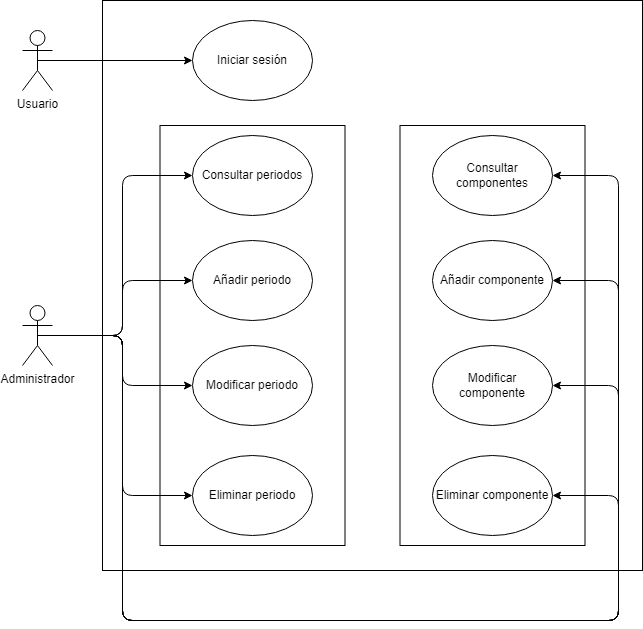
\includegraphics[scale=0.7]{casos-uso-admin}}
\caption{Diagrama de casos de uso de la administración del museo}
\end{figure}

\begin{table}[htbp]
  \centering
  \caption{Especificación Caso de Uso 3}
    \begin{tabular}{p{20.855em}r}
\cmidrule{1-1}    \rowcolor[rgb]{ .949,  .949,  .949} \multicolumn{1}{p{20.855em}}{\textbf{Nombre del caso de uso}} & \multicolumn{1}{r}{\cellcolor[rgb]{ 1,  1,  1}} \\
\cmidrule{1-1}    \multicolumn{1}{p{20.855em}}{Iniciar sesión} & \multicolumn{1}{r}{} \\
    \midrule
    \rowcolor[rgb]{ .949,  .949,  .949} \multicolumn{2}{p{31.64em}}{\textbf{Descripción}} \\
    \midrule
    \multicolumn{2}{p{31.64em}}{Un usuario puede iniciar sesión en la aplicación para acceder a esta como administrador.} \\
    \bottomrule
    \end{tabular}%
  \label{espec_caso_uso_3}%
  \vspace{-2mm}
\end{table}%

\begin{table}[htbp]
  \centering
  \caption{Especificación Caso de Uso 4}
    \begin{tabular}{p{20.855em}r}
\cmidrule{1-1}    \rowcolor[rgb]{ .949,  .949,  .949} \multicolumn{1}{p{20.855em}}{\textbf{Nombre del caso de uso}} & \multicolumn{1}{r}{\cellcolor[rgb]{ 1,  1,  1}} \\
\cmidrule{1-1}    \multicolumn{1}{p{20.855em}}{Consultar periodos} & \multicolumn{1}{r}{} \\
    \midrule
    \rowcolor[rgb]{ .949,  .949,  .949} \multicolumn{2}{p{31.64em}}{\textbf{Descripción}} \\
    \midrule
    \multicolumn{2}{p{31.64em}}{El administrador puede consultar los periodos existentes en el sistema.} \\
    \bottomrule
    \end{tabular}%
  \label{espec_caso_uso_4}%
  \vspace{-2mm}
\end{table}%

\begin{table}[htbp]
  \centering
  \caption{Especificación Caso de Uso 5}
    \begin{tabular}{p{20.855em}r}
\cmidrule{1-1}    \rowcolor[rgb]{ .949,  .949,  .949} \multicolumn{1}{p{20.855em}}{\textbf{Nombre del caso de uso}} & \multicolumn{1}{r}{\cellcolor[rgb]{ 1,  1,  1}} \\
\cmidrule{1-1}    \multicolumn{1}{p{20.855em}}{Añadir periodo} & \multicolumn{1}{r}{} \\
    \midrule
    \rowcolor[rgb]{ .949,  .949,  .949} \multicolumn{2}{p{31.64em}}{\textbf{Descripción}} \\
    \midrule
    \multicolumn{2}{p{31.64em}}{El administrador puede añadir periodos a la base de datos del sistema.} \\
    \bottomrule
    \end{tabular}%
  \label{espec_caso_uso_5}%
  \vspace{-2mm}
\end{table}%

\begin{table}[htbp]
  \centering
  \caption{Especificación Caso de Uso 6}
    \begin{tabular}{p{20.855em}r}
\cmidrule{1-1}    \rowcolor[rgb]{ .949,  .949,  .949} \multicolumn{1}{p{20.855em}}{\textbf{Nombre del caso de uso}} & \multicolumn{1}{r}{\cellcolor[rgb]{ 1,  1,  1}} \\
\cmidrule{1-1}    \multicolumn{1}{p{20.855em}}{Modificar periodo} & \multicolumn{1}{r}{} \\
    \midrule
    \rowcolor[rgb]{ .949,  .949,  .949} \multicolumn{2}{p{31.64em}}{\textbf{Descripción}} \\
    \midrule
    \multicolumn{2}{p{31.64em}}{El administrador puede modificar los periodos existentes en la base de datos del sistema.} \\
    \bottomrule
    \end{tabular}%
  \label{espec_caso_uso_6}%
  \vspace{-2mm}
\end{table}%

\begin{table}[htbp]
  \centering
  \caption{Especificación Caso de Uso 7}
    \begin{tabular}{p{20.855em}r}
\cmidrule{1-1}    \rowcolor[rgb]{ .949,  .949,  .949} \multicolumn{1}{p{20.855em}}{\textbf{Nombre del caso de uso}} & \multicolumn{1}{r}{\cellcolor[rgb]{ 1,  1,  1}} \\
\cmidrule{1-1}    \multicolumn{1}{p{20.855em}}{Eliminar periodo} & \multicolumn{1}{r}{} \\
    \midrule
    \rowcolor[rgb]{ .949,  .949,  .949} \multicolumn{2}{p{31.64em}}{\textbf{Descripción}} \\
    \midrule
    \multicolumn{2}{p{31.64em}}{El administrador puede eliminar los periodos existentes en la base de datos del sistema.} \\
    \bottomrule
    \end{tabular}%
  \label{espec_caso_uso_7}%
  \vspace{-2mm}
\end{table}%

\begin{table}[htbp]
  \centering
  \caption{Especificación Caso de Uso 8}
    \begin{tabular}{p{20.855em}r}
\cmidrule{1-1}    \rowcolor[rgb]{ .949,  .949,  .949} \multicolumn{1}{p{20.855em}}{\textbf{Nombre del caso de uso}} & \multicolumn{1}{r}{\cellcolor[rgb]{ 1,  1,  1}} \\
\cmidrule{1-1}    \multicolumn{1}{p{20.855em}}{Consultar componentes} & \multicolumn{1}{r}{} \\
    \midrule
    \rowcolor[rgb]{ .949,  .949,  .949} \multicolumn{2}{p{31.64em}}{\textbf{Descripción}} \\
    \midrule
    \multicolumn{2}{p{31.64em}}{El administrador puede consultar los componentes existentes en el sistema.} \\
    \bottomrule
    \end{tabular}%
  \label{espec_caso_uso_8}%
  \vspace{-2mm}
\end{table}%

\begin{table}[htbp]
  \centering
  \caption{Especificación Caso de Uso 9}
    \begin{tabular}{p{20.855em}r}
\cmidrule{1-1}    \rowcolor[rgb]{ .949,  .949,  .949} \multicolumn{1}{p{20.855em}}{\textbf{Nombre del caso de uso}} & \multicolumn{1}{r}{\cellcolor[rgb]{ 1,  1,  1}} \\
\cmidrule{1-1}    \multicolumn{1}{p{20.855em}}{Añadir componente} & \multicolumn{1}{r}{} \\
    \midrule
    \rowcolor[rgb]{ .949,  .949,  .949} \multicolumn{2}{p{31.64em}}{\textbf{Descripción}} \\
    \midrule
    \multicolumn{2}{p{31.64em}}{El administrador puede añadir componentes a los periodos existentes en la base de datos del sistema.} \\
    \bottomrule
    \end{tabular}%
  \label{espec_caso_uso_9}%
  \vspace{-2mm}
\end{table}%

\begin{table}[htbp]
  \centering
  \caption{Especificación Caso de Uso 10}
    \begin{tabular}{p{20.855em}r}
\cmidrule{1-1}    \rowcolor[rgb]{ .949,  .949,  .949} \multicolumn{1}{p{20.855em}}{\textbf{Nombre del caso de uso}} & \multicolumn{1}{r}{\cellcolor[rgb]{ 1,  1,  1}} \\
\cmidrule{1-1}    \multicolumn{1}{p{20.855em}}{Modificar componente} & \multicolumn{1}{r}{} \\
    \midrule
    \rowcolor[rgb]{ .949,  .949,  .949} \multicolumn{2}{p{31.64em}}{\textbf{Descripción}} \\
    \midrule
    \multicolumn{2}{p{31.64em}}{El administrador puede modificar los componentes existentes en la base de datos del sistema.} \\
    \bottomrule
    \end{tabular}%
  \label{espec_caso_uso_10}%
  \vspace{-2mm}
\end{table}%

\begin{table}[htbp]
  \centering
  \caption{Especificación Caso de Uso 11}
    \begin{tabular}{p{20.855em}r}
\cmidrule{1-1}    \rowcolor[rgb]{ .949,  .949,  .949} \multicolumn{1}{p{20.855em}}{\textbf{Nombre del caso de uso}} & \multicolumn{1}{r}{\cellcolor[rgb]{ 1,  1,  1}} \\
\cmidrule{1-1}    \multicolumn{1}{p{20.855em}}{Eliminar componente} & \multicolumn{1}{r}{} \\
    \midrule
    \rowcolor[rgb]{ .949,  .949,  .949} \multicolumn{2}{p{31.64em}}{\textbf{Descripción}} \\
    \midrule
    \multicolumn{2}{p{31.64em}}{El administrador puede eliminar los componentes existentes en la base de datos del sistema.} \\
    \bottomrule
    \end{tabular}%
  \label{espec_caso_uso_11}%
  \vspace{-2mm}
\end{table}%